\documentclass[8pt,aspectratio=169]{beamer}
\usetheme{Madrid}
\usepackage{graphicx}
\usepackage{booktabs}
\usepackage{adjustbox}
\usepackage{multicol}
\usepackage{amsmath}
\usepackage{amssymb}
\usepackage{tikz}
\usepackage{hyperref}
\usepackage{algorithm}
\usepackage{algorithmic}
\usepackage{colortbl}
\usepackage{pgfplots}
\pgfplotsset{compat=1.18}

% TikZ libraries for comics, diagrams, stakeholder maps
\usetikzlibrary{arrows.meta,positioning,shapes.callouts,shapes.geometric,decorations.pathreplacing}

% Color definitions
\definecolor{mlblue}{RGB}{0,102,204}
\definecolor{mlpurple}{RGB}{51,51,178}
\definecolor{mllavender}{RGB}{173,173,224}
\definecolor{mllavender2}{RGB}{193,193,232}
\definecolor{mllavender3}{RGB}{204,204,235}
\definecolor{mllavender4}{RGB}{214,214,239}
\definecolor{mlorange}{RGB}{255, 127, 14}
\definecolor{mlgreen}{RGB}{44, 160, 44}
\definecolor{mlred}{RGB}{214, 39, 40}
\definecolor{mlgray}{RGB}{127, 127, 127}
\definecolor{lightgray}{RGB}{240, 240, 240}
\definecolor{midgray}{RGB}{180, 180, 180}

% NEW COLORS for mini-lecture
\definecolor{dfteal}{RGB}{0,128,128}
\definecolor{dfred}{RGB}{180,30,30}

% Backward compatibility
\colorlet{MLPurple}{mlpurple}
\colorlet{MLBlue}{mlblue}
\colorlet{MLOrange}{mlorange}
\colorlet{MLGreen}{mlgreen}
\colorlet{MLRed}{mlred}
\colorlet{MLLavender}{mllavender}
\colorlet{MLGray}{mlgray}

% Theme colors (exact Madrid settings)
\setbeamercolor{palette primary}{bg=mllavender3,fg=mlpurple}
\setbeamercolor{palette secondary}{bg=mllavender2,fg=mlpurple}
\setbeamercolor{palette tertiary}{bg=mllavender,fg=white}
\setbeamercolor{palette quaternary}{bg=mlpurple,fg=white}
\setbeamercolor{structure}{fg=mlpurple}
\setbeamercolor{section in toc}{fg=mlpurple}
\setbeamercolor{subsection in toc}{fg=mlblue}
\setbeamercolor{title}{fg=mlpurple}
\setbeamercolor{frametitle}{fg=mlpurple,bg=mllavender3}
\setbeamercolor{block title}{bg=mllavender2,fg=mlpurple}
\setbeamercolor{block body}{bg=mllavender4,fg=black}
\setbeamertemplate{navigation symbols}{}
\setbeamertemplate{itemize items}[circle]
\setbeamertemplate{enumerate items}[default]
\setbeamersize{text margin left=5mm,text margin right=5mm}

% Footer
\setbeamertemplate{footline}{
  \leavevmode%
  \hbox{%
    \begin{beamercolorbox}[wd=.333333\paperwidth,ht=2.25ex,dp=1ex,center]{author in head/foot}%
      \usebeamerfont{author in head/foot}Methods and Algorithms
    \end{beamercolorbox}%
    \begin{beamercolorbox}[wd=.333333\paperwidth,ht=2.25ex,dp=1ex,center]{title in head/foot}%
      \usebeamerfont{title in head/foot}MSc Data Science
    \end{beamercolorbox}%
    \begin{beamercolorbox}[wd=.333333\paperwidth,ht=2.25ex,dp=1ex,right]{date in head/foot}%
      \usebeamerfont{date in head/foot}\insertframenumber{} / \inserttotalframenumber\hspace*{2ex}
    \end{beamercolorbox}}%
  \vskip0pt%
}

\newcommand{\bottomnote}[1]{%
\vfill
\vspace{-2mm}
\textcolor{mllavender2}{\rule{\textwidth}{0.4pt}}
\vspace{1mm}
\footnotesize
\textbf{#1}
}

\newenvironment{compactlist}{%
  \begin{itemize}%
    \setlength{\itemsep}{2pt}%
    \setlength{\parskip}{0pt}%
    \setlength{\parsep}{0pt}%
}{%
  \end{itemize}%
}

\newcommand{\highlight}[1]{\textcolor{mlorange}{\textbf{#1}}}
\newcommand{\mathbold}[1]{\boldsymbol{#1}}

\title[PCA \& t-SNE Mini-Lecture]{PCA \& t-SNE}
\subtitle{Mini-Lecture: Seeing the Big Picture in High Dimensions}
\author{Methods \& Algorithms}
\date{MSc Data Science -- Spring 2026}

\begin{document}

%% ================================================================
%% SLIDE 1: Title Page
%% ================================================================
\begin{frame}[plain]
\titlepage
\end{frame}

%% ================================================================
%% SLIDE 2: Opening XKCD
%% ================================================================
\begin{frame}[t]{When You Have Too Many Dimensions to Plot}
\begin{center}
\includegraphics[width=0.6\textwidth,height=0.7\textheight,keepaspectratio]{images/2048_curve_fitting.png}
\end{center}

\bottomnote{XKCD \#2048 by Randall Munroe (CC BY-NC 2.5)}
\end{frame}

%% ================================================================
%% SLIDE 3: The Curse of Dimensionality
%% ================================================================
\begin{frame}[t]{The Curse of Dimensionality}
\begin{columns}[T]
\column{0.55\textwidth}
\small
\textbf{Why High-Dimensional Data Is Hard}
\begin{compactlist}
\item In high dimensions, all points become equally distant -- nearest-neighbor methods break down
\item A dataset that seems dense in 2D becomes sparse in 100D
\item Visualization is impossible beyond 3 dimensions
\item Many features are redundant or correlated -- we need to compress without losing structure
\end{compactlist}

\begin{block}{Key Question}
\scriptsize Can we reduce 100 features to 2--3 while preserving the important patterns?
\end{block}

\column{0.42\textwidth}
\vspace{4mm}
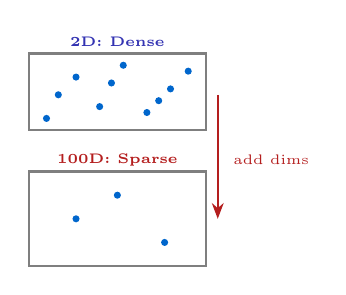
\begin{tikzpicture}[scale=0.75]
% 2D: dense
\node[font=\tiny\bfseries, mlpurple] at (1.5,4.5) {2D: Dense};
\draw[mlgray, thick] (0,3) rectangle (3,4.3);
\foreach \x/\y in {0.3/3.2, 0.8/3.9, 1.2/3.4, 1.6/4.1, 2.0/3.3, 2.4/3.7, 2.7/4.0, 0.5/3.6, 1.4/3.8, 2.2/3.5} {
  \fill[mlblue] (\x,\y) circle (0.06);
}
% 100D: sparse
\node[font=\tiny\bfseries, dfred] at (1.5,2.5) {100D: Sparse};
\draw[mlgray, thick] (0,0.7) rectangle (3,2.3);
\fill[mlblue] (0.8,1.5) circle (0.06);
\fill[mlblue] (2.3,1.1) circle (0.06);
\fill[mlblue] (1.5,1.9) circle (0.06);
% Arrow
\draw[-{Stealth[length=2mm]}, dfred, thick] (3.2,3.6) -- (3.2,1.5);
\node[font=\tiny, dfred, right] at (3.3,2.5) {add dims};
\end{tikzpicture}
\end{columns}

\bottomnote{Bellman (1961) coined ``curse of dimensionality'' -- the volume of space grows exponentially with dimensions}
\end{frame}

%% ================================================================
%% SLIDE 4: PCA Intuition
%% ================================================================
\begin{frame}[t]{PCA: Find the Directions of Maximum Variance}
\begin{columns}[T]
\column{0.55\textwidth}
\small
\textbf{Principal Component Analysis}
\begin{compactlist}
\item \highlight{Step 1}: Center the data (subtract the mean)
\item \highlight{Step 2}: Find the direction of maximum variance -- that is PC1
\item \highlight{Step 3}: Find the next orthogonal direction of maximum variance -- that is PC2
\item Project data onto these new axes to reduce dimensions
\end{compactlist}

\vspace{1mm}
\scriptsize Mathematically: eigendecomposition of the covariance matrix $\Sigma = \frac{1}{n}X^TX$.

\begin{block}{Insight}
\scriptsize PCA is a rotation -- it does not discard data, it reorders it by importance (variance).
\end{block}

\column{0.42\textwidth}
\vspace{2mm}
\includegraphics[width=0.55\textwidth]{02_principal_components/chart.pdf}
\end{columns}

\bottomnote{PCA preserves global structure (variance) -- it finds the best linear summary of your data}
\end{frame}

%% ================================================================
%% SLIDE 5: How Many Components?
%% ================================================================
\begin{frame}[t]{How Many Components Do We Keep?}
\begin{columns}[T]
\column{0.55\textwidth}
\small
\textbf{The Scree Plot}
\begin{compactlist}
\item Plot explained variance ratio for each component
\item Look for the ``elbow'' -- where additional components add little
\item Rule of thumb: keep enough components to explain 90--95\% of total variance
\item Alternatively, use cross-validation on a downstream task
\end{compactlist}

\begin{block}{Insight}
\scriptsize If 3 components explain 95\% of variance in 50 features, you have compressed 50D to 3D with minimal information loss.
\end{block}

\column{0.42\textwidth}
\vspace{2mm}
\includegraphics[width=0.55\textwidth]{01_scree_plot/chart.pdf}
\end{columns}

\bottomnote{The scree plot is named after the geological term for rubble at the base of a cliff -- you stop where the ``cliff'' flattens}
\end{frame}

%% ================================================================
%% SLIDE 6: t-SNE
%% ================================================================
\begin{frame}[t]{t-SNE: Preserving Neighborhoods in 2D}
\begin{columns}[T]
\column{0.55\textwidth}
\small
\textbf{When Linear Projection Fails}
\begin{compactlist}
\item \highlight{t-SNE} (van der Maaten \& Hinton, 2008) is a non-linear method for visualization
\item Converts high-D distances to probabilities, then matches them in 2D
\item Preserves \highlight{local structure}: nearby points stay nearby
\item Warning: global distances are not meaningful in t-SNE plots
\end{compactlist}

\begin{block}{Insight}
\scriptsize t-SNE is for looking at your data, not for feeding into a model. Use PCA for preprocessing, t-SNE for visualization.
\end{block}

\column{0.42\textwidth}
\vspace{4mm}
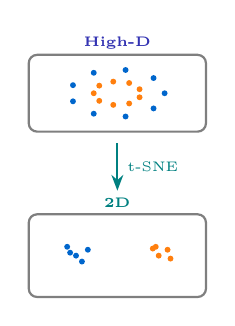
\begin{tikzpicture}[scale=0.75]
% High-D box
\node[font=\tiny\bfseries, mlpurple] at (1.5,4.5) {High-D};
\draw[mlgray, thick, rounded corners=3pt] (0,3.0) rectangle (3,4.3);
% Interleaved clusters (hard to separate linearly)
\foreach \a in {0,40,...,320} {
  \fill[mlblue] ({1.5+0.8*cos(\a)},{3.65+0.4*sin(\a)}) circle (0.05);
}
\foreach \a in {20,60,...,340} {
  \fill[mlorange] ({1.5+0.4*cos(\a)},{3.65+0.2*sin(\a)}) circle (0.05);
}
% Arrow
\draw[-{Stealth[length=2mm]}, dfteal, thick] (1.5,2.8) -- (1.5,2.0) node[midway, right, font=\tiny] {t-SNE};
% 2D box
\node[font=\tiny\bfseries, dfteal] at (1.5,1.8) {2D};
\draw[mlgray, thick, rounded corners=3pt] (0,0.2) rectangle (3,1.6);
% Separated clusters
\foreach \dx/\dy in {0/0, 0.2/0.1, -0.15/0.15, 0.1/-0.1, -0.1/0.05} {
  \fill[mlblue] (0.8+\dx, 0.9+\dy) circle (0.05);
}
\foreach \dx/\dy in {0/0, 0.15/0.1, -0.1/0.12, 0.2/-0.05, -0.05/0.15} {
  \fill[mlorange] (2.2+\dx, 0.9+\dy) circle (0.05);
}
\end{tikzpicture}
\end{columns}

\bottomnote{t-SNE clusters are real (local structure is preserved), but cluster distances and sizes are not -- never interpret gaps}
\end{frame}

%% ================================================================
%% SLIDE 7: Perplexity
%% ================================================================
\begin{frame}[t]{Perplexity: t-SNE's Key Hyperparameter}
\begin{columns}[T]
\column{0.55\textwidth}
\small
\textbf{Balancing Local vs Global Structure}
\begin{compactlist}
\item \highlight{Perplexity} $\approx$ effective number of neighbors each point considers
\item Low perplexity (5--10): tight local clusters, noisy global layout
\item High perplexity (30--50): smoother layout, may merge distinct groups
\item Always try multiple perplexity values before drawing conclusions
\end{compactlist}

\begin{block}{Insight}
\scriptsize There is no ``correct'' perplexity. If your conclusions change with perplexity, they are artifacts of the method, not real structure.
\end{block}

\column{0.42\textwidth}
\vspace{2mm}
\footnotesize
\begin{tabular}{@{}l p{3.0cm}@{}}
\toprule
\textbf{Perplexity} & \textbf{Behavior} \\
\midrule
\rowcolor{mllavender4}
5 & Very local, fragmented clusters \\
30 & Balanced (default in sklearn) \\
\rowcolor{mllavender4}
50 & Smoother, global trends visible \\
100+ & Over-smoothed, clusters merge \\
\bottomrule
\end{tabular}

\vspace{3mm}
\scriptsize \textbf{Rule of thumb:} perplexity should be smaller than $n/3$ where $n$ is the number of data points.
\end{columns}

\bottomnote{Wattenberg et al.\ (2016) ``How to Use t-SNE Effectively'' -- essential reading before interpreting t-SNE plots}
\end{frame}

%% ================================================================
%% SLIDE 8: PCA vs t-SNE
%% ================================================================
\begin{frame}[t]{PCA vs t-SNE: When to Use Which?}
\begin{columns}[T]
\column{0.95\textwidth}
\small
\textbf{Comparison Table}

\vspace{2mm}
\footnotesize
\begin{tabular}{@{}l c c@{}}
\toprule
\textbf{Property} & \textbf{\textcolor{dfteal}{PCA}} & \textbf{\textcolor{mlpurple}{t-SNE}} \\
\midrule
\rowcolor{mllavender4}
Type & Linear & Non-linear \\
Preserves & Global variance & Local neighborhoods \\
\rowcolor{mllavender4}
Invertible & Yes (reconstruct data) & No \\
Speed & Fast ($O(np^2)$) & Slow ($O(n^2)$) \\
\rowcolor{mllavender4}
Deterministic & Yes & No (random initialization) \\
Use for modeling & Yes (preprocessing) & No (visualization only) \\
\rowcolor{mllavender4}
Interpretable axes & Yes (loadings) & No \\
\bottomrule
\end{tabular}

\vspace{3mm}
\begin{block}{Practical Advice}
\scriptsize Run PCA first to reduce to 30--50 dimensions, then apply t-SNE for visualization. This is faster and more stable than running t-SNE on raw high-D data.
\end{block}
\end{columns}

\bottomnote{PCA + t-SNE pipeline: PCA for compression and denoising, t-SNE for the final 2D visualization}
\end{frame}

%% ================================================================
%% SLIDE 9: Finance Application
%% ================================================================
\begin{frame}[t]{Finance Application: Yield Curve PCA}
\begin{columns}[T]
\column{0.55\textwidth}
\small
\textbf{The Three Factors of Interest Rates}
\begin{compactlist}
\item PCA on yield curve data (1Y, 2Y, 5Y, 10Y, 30Y rates) reveals 3 dominant components
\item \highlight{PC1 ($\sim$85\%)}: Level -- parallel shift of all rates
\item \highlight{PC2 ($\sim$10\%)}: Slope -- short vs long rates diverge
\item \highlight{PC3 ($\sim$3\%)}: Curvature -- belly of the curve moves
\end{compactlist}

\begin{block}{Insight}
\scriptsize 3 components explain 98\% of yield curve variation. Fixed income risk management is built on this PCA decomposition.
\end{block}

\column{0.42\textwidth}
\vspace{2mm}
\footnotesize
\fcolorbox{mlpurple}{mllavender4}{\parbox{0.85\columnwidth}{%
\textbf{Portfolio Risk with PCA:}

\vspace{2mm}
Instead of tracking 10 maturities, track 3 factor exposures:

\vspace{2mm}
$\Delta P \approx D_1 \cdot \Delta\text{PC1}$

$\quad + D_2 \cdot \Delta\text{PC2}$

$\quad + D_3 \cdot \Delta\text{PC3}$

\vspace{2mm}
\textbf{$D_k$}: factor duration (sensitivity to factor $k$)
}}
\end{columns}

\bottomnote{Litterman \& Scheinkman (1991) showed that 3 PCA factors explain $>$98\% of US Treasury yield curve movements}
\end{frame}

%% ================================================================
%% SLIDE 10: Summary
%% ================================================================
\begin{frame}[t]{Summary: Dimensionality Reduction in 4 Takeaways}
\begin{columns}[T]
\column{0.95\textwidth}
\small
\begin{enumerate}
\setlength{\itemsep}{6pt}
\item \highlight{Curse of dimensionality}: high-D data is sparse, distances become meaningless, and visualization is impossible without reduction
\item \highlight{PCA}: linear, fast, invertible -- finds directions of maximum variance. Use for preprocessing and interpretable compression.
\item \highlight{t-SNE}: non-linear, slow, for visualization only -- preserves local neighborhoods but not global distances. Always try multiple perplexity values.
\item \highlight{Finance}: yield curve PCA (level, slope, curvature) reduces 10+ maturities to 3 factors explaining 98\% of variance
\end{enumerate}

\vspace{4mm}
\begin{block}{Next Steps}
\scriptsize Explore the deep dive slides for eigenvalue derivations, kernel PCA, and UMAP. Try the Jupyter notebook to run PCA on real financial data.
\end{block}
\end{columns}

\bottomnote{PCA is a tool; t-SNE is a lens. Use PCA to simplify your data, use t-SNE to look at it.}
\end{frame}

\end{document}
